\documentclass[column,brazilian,12pt,a4paper,final]{article}
\usepackage[brazil]{babel}
%\usepackage{nonfloat}
\usepackage[utf8]{inputenc}
\usepackage{multicol}
\usepackage{hyperref}
\usepackage[pdftex]{color,graphicx}
\usepackage{geometry}
\usepackage{amsmath}
\usepackage{caption}

 \geometry{
 a4paper,
 total={170mm,257mm},
 left=20mm,
 top=20mm,
 }
 \usepackage{ragged2e}
\usepackage{fancyhdr}
\usepackage{caption}[=v1]
\usepackage{xcolor}
\usepackage{circuitikz}
\pagestyle{plain}
\fancyhead{}
\lhead{
\includegraphics[width=1.5cm]{logoufrgs}}
\rhead{
\includegraphics[width=0.8cm]{logoif}}
\fancyfoot{}
\fancyhead[C]{\footnotesize Física Experimental III $\bullet$ 2025/1}
\fancyfoot[RO]{\thepage}
\usepackage{float}
\usepackage{setspace}
\usepackage{fancyref}


\title{}
\author{Autores: \\ Lucas Assis Paulino da Silva - 590174 \\Lucas Bertazo de Deus Félix - 587064
 \\ Pedro Henrique Reis de Oliveira - 590908 \\ IF-UFRGS}
\date{Abril 2025}

\begin{document}
\maketitle
\thispagestyle{fancy}

\section*{Resumo}
\paragraph{}
[...]

\section{Introdução}
\paragraph{}
[...]

\section{Embasamento Teórico}
\paragraph{}
[...]

\section{Material Utilizado}
\begin{itemize}
    \item Fios, conectores, circuito
    \item Multímetro Minipa® ET-2075B (Precisão 0,001V e 0,01$\mu$F)
    \item Fonte Elétrica - IF UFRGS
    \item Capacitor (23,28$\mu$F)
    \item Cronômetro (Precisão 0,01s)
    \item Smartphone com câmera (Para gravação do vídeo)
\end{itemize}

\section{Procedimentos e Montagem}
\paragraph{}
[...]

\section{Dados Experimentais}
\paragraph{}
Os dados de tensão ($V$) em função do tempo ($t$) foram adquiridos com o auxílio de um osciloscópio. Para garantir a reprodutibilidade e avaliar a consistência dos resultados, registramos X medições para cada um dos três cenários experimentais definidos: com a bobina geradora e o ímã, com a bobina geradora e a bobina detectora, sem o núcleo de ferro e por último com a bobina geradora e a bobina detectora, com a inserção do núcleo de ferro.

A seguir, apresentamos um gráfico representativo de cada cenário. Para facilitar a visualização do evento de indução, os gráficos foram plotados no intervalo de tempo específico onde o pulso de tensão ocorre. A análise quantitativa subsequente focará na determinação do fluxo a partir da integral da curva V(t). O conjunto completo de dados brutos para todas as Y medições pode ser consultado no Apêndice.

\begin{figure}[H]
    \centering
    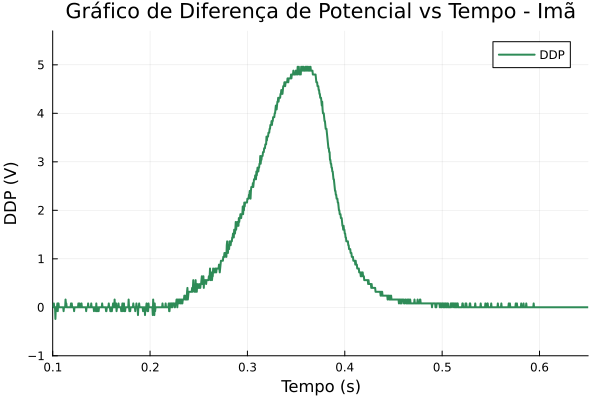
\includegraphics[width=0.8\textwidth]{figuras/grafico_diferenca_potencial - 1.png}
    \caption{Gráfico de tensão versus tempo com a bobina geradora e o imã.}
    \label{fig:grafico1}
\end{figure}
\begin{figure}[H]
    \centering
    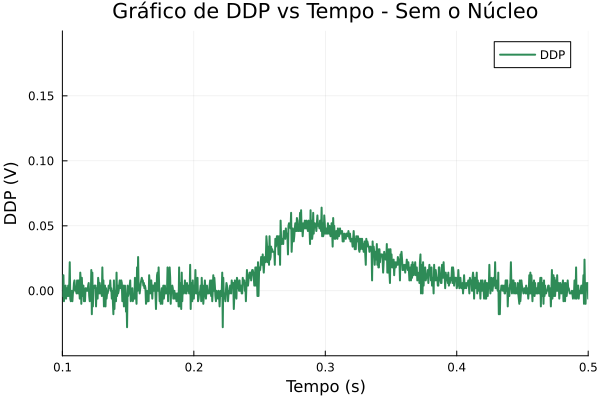
\includegraphics[width=0.8\textwidth]{figuras/grafico_diferenca_potencial - 2.png}
    \caption{Gráfico de tensão versus tempo com a bobina geradora e o detector sem o núcleo de ferro.}
    \label{fig:grafico2}
\end{figure}
\begin{figure}[H]
    \centering
    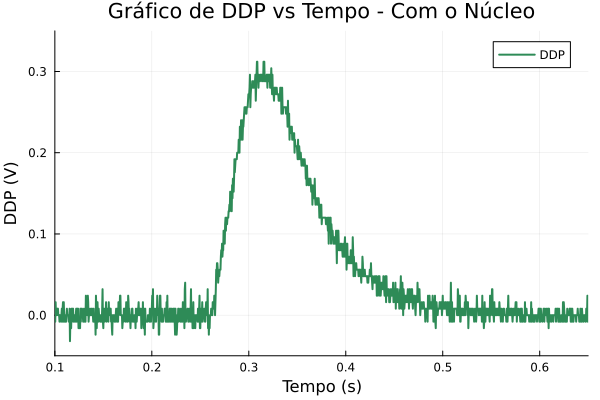
\includegraphics[width=0.8\textwidth]{figuras/grafico_diferenca_potencial - 3.png}
    \caption{Gráfico de tensão versus tempo com a bobina geradora e o detector com o núcleo de ferro.}
    \label{fig:grafico3}
\end{figure}



\section{Análise de Dados}
De posse dos dados experimentais, utilizamos a integração numérica com o método do trapézio para calcular o fluxo magnético $\Phi$ através da bobina detectora. A partir da equação (14) desenvolvida na seção de embasamento teórico, podemos expressar o fluxo magnético experimental como o resultado da integral da curva de tensão em função do tempo dividida pelo número de voltas $N$ da bobina detectora. 
O resultado esperado é que o valor dessa integral seja constante entre as medições 
\section{Conclusão}
[...]

\begin{thebibliography}{99}

\bibitem{}
Processamento de dados e produção de gráficos:
\url{https://github.com/pedro-hro/Relatorio_3-ExperimentalIII}
\bibitem{}
RUTH W. CHABBAY. Matter and Interactions 4th Edition - Matter and Interactions, 4th Edition. WILEY, 2015.
\bibitem{}
NUSSENZVEIG, H. Moysés. {\em Curso de Física Básica - Mecânica}. 5ª ed., vol. 3. São Paulo: Edgard Blücher Ltda, 2013.
\bibitem{}
Schechner, S. J. (2015). The Art of Making Leyden Jars and Batteries according to Benjamin Franklin. ERittenhouse, 26. https://saraschechner.scholars.harvard.edu/publications/art-making-leyden-jars-and-batteries-according-benjamin-franklin


\end{thebibliography}

\section*{Apêndice}
\paragraph{}
\section*{Gráficos de DDP vs Tempo}
\begin{center}
\begin{multicols}{2}

\begin{figure}[H]
    \centering
    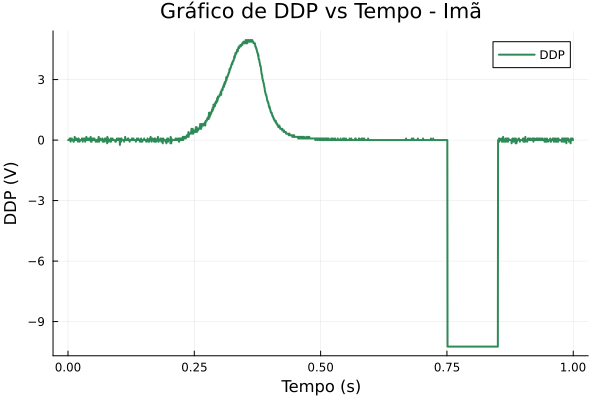
\includegraphics[width=1.0\linewidth]{figuras/grafico_dados1_F0002CH1.png}
\end{figure}

\begin{figure}[H]
    \centering
    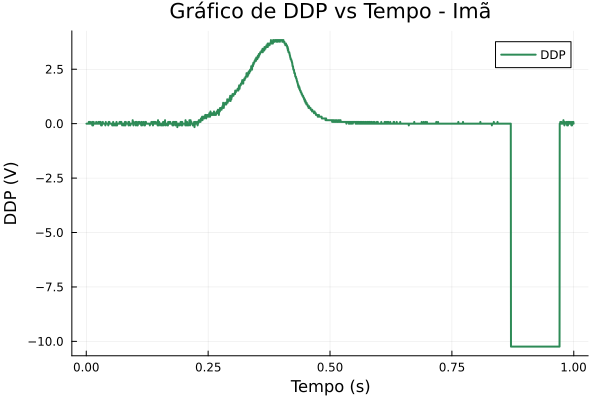
\includegraphics[width=1.0\linewidth]{figuras/grafico_dados1_F0003CH1.png}
\end{figure}

\begin{figure}[H]
    \centering
    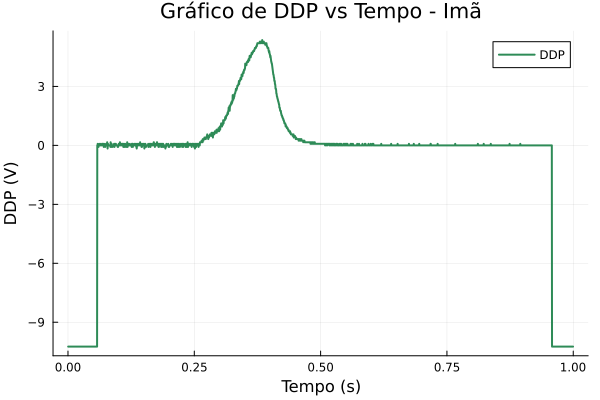
\includegraphics[width=1.0\linewidth]{figuras/grafico_dados1_F0004CH1.png}
\end{figure}

\begin{figure}[H]
    \centering
    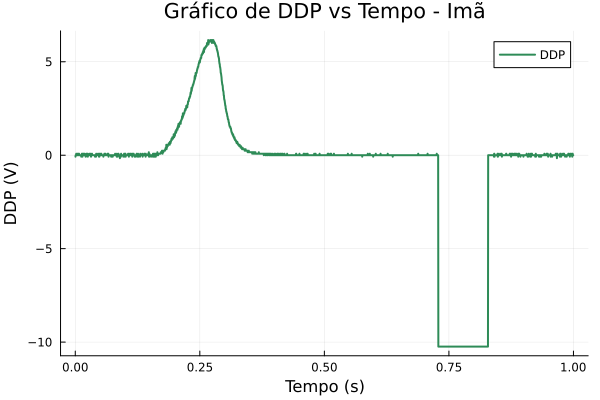
\includegraphics[width=1.0\linewidth]{figuras/grafico_dados1_F0005CH1.png}
\end{figure}

\begin{figure}[H]
    \centering
    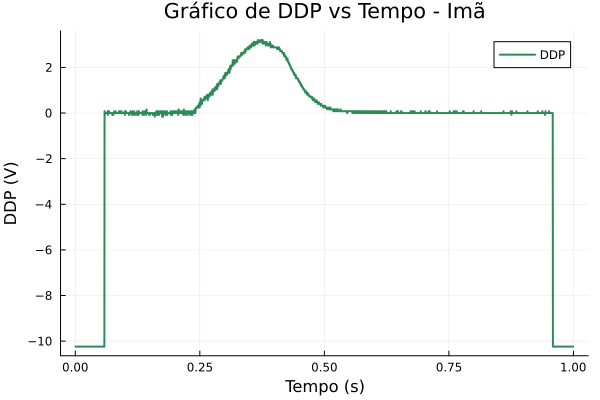
\includegraphics[width=1.0\linewidth]{figuras/grafico_dados1_F0006CH1.png}
\end{figure}

\begin{figure}[H]
    \centering
    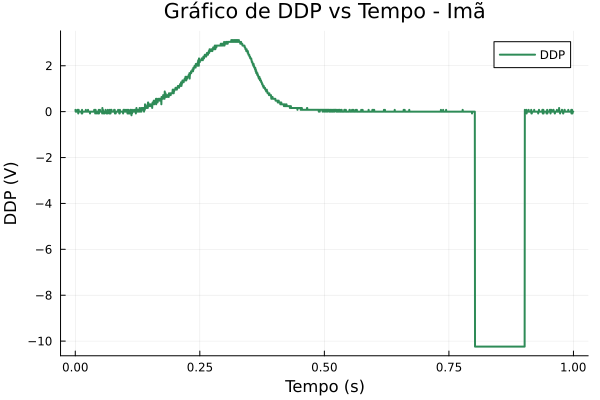
\includegraphics[width=1.0\linewidth]{figuras/grafico_dados1_F0007CH1.png}
\end{figure}

\begin{figure}[H]
    \centering
    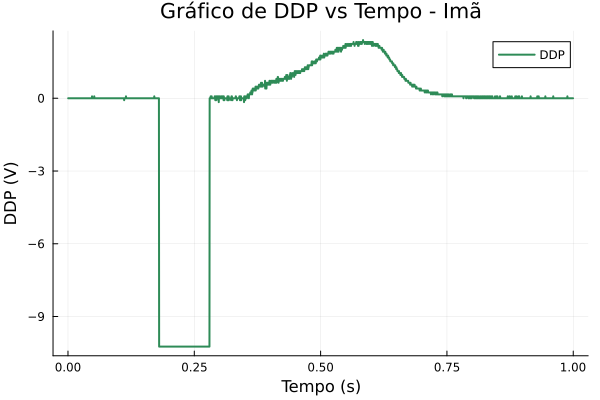
\includegraphics[width=1.0\linewidth]{figuras/grafico_dados1_F0008CH1.png}
\end{figure}

\begin{figure}[H]
    \centering
    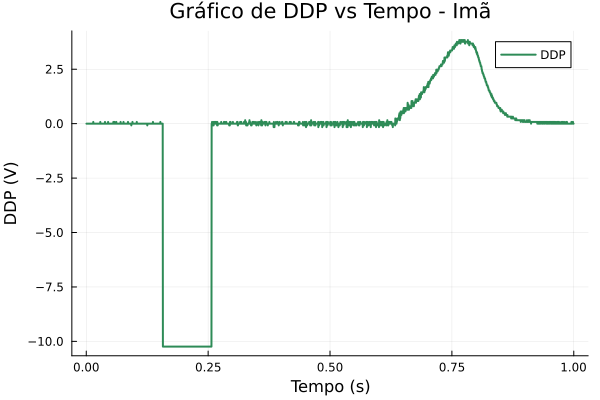
\includegraphics[width=1.0\linewidth]{figuras/grafico_dados1_F0009CH1.png}
\end{figure}

\begin{figure}[H]
    \centering
    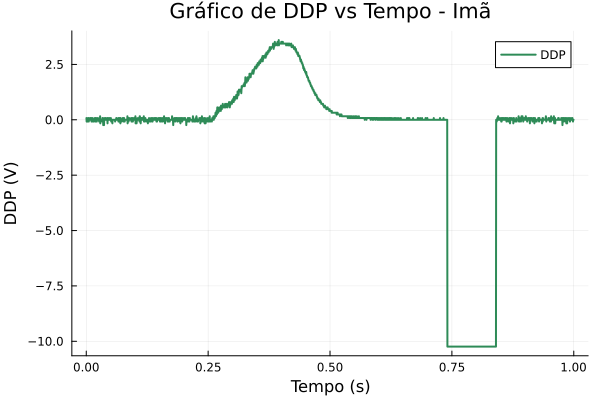
\includegraphics[width=1.0\linewidth]{figuras/grafico_dados1_F0010CH1.png}
\end{figure}

\begin{figure}[H]
    \centering
    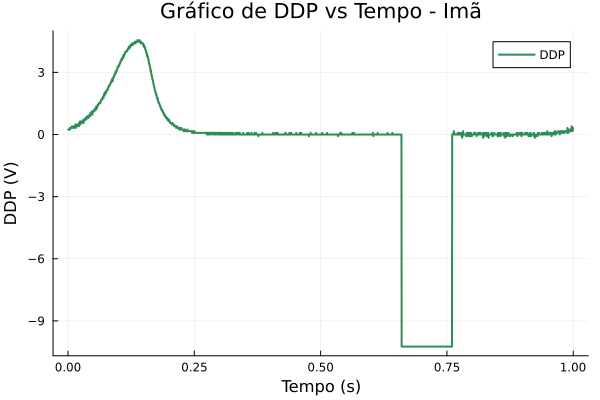
\includegraphics[width=1.0\linewidth]{figuras/grafico_dados1_F0011CH1.png}
\end{figure}

\begin{figure}[H]
    \centering
    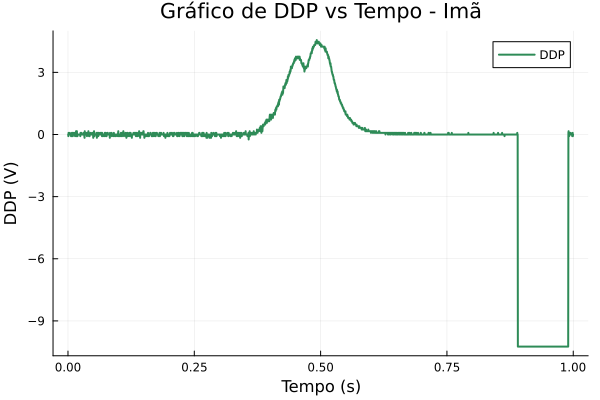
\includegraphics[width=1.0\linewidth]{figuras/grafico_dados1_F0012CH1.png}
\end{figure}

\begin{figure}[H]
    \centering
    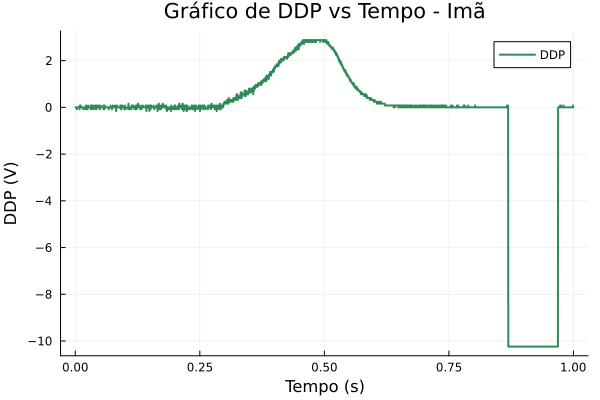
\includegraphics[width=1.0\linewidth]{figuras/grafico_dados1_F0013CH1.png}
\end{figure}

\begin{figure}[H]
    \centering
    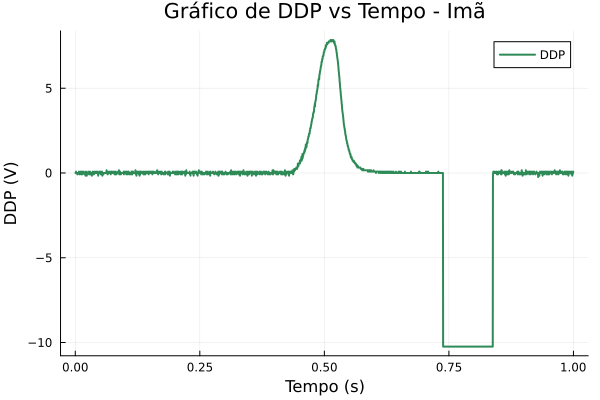
\includegraphics[width=1.0\linewidth]{figuras/grafico_dados1_F0014CH1.png}
\end{figure}

\begin{figure}[H]
    \centering
    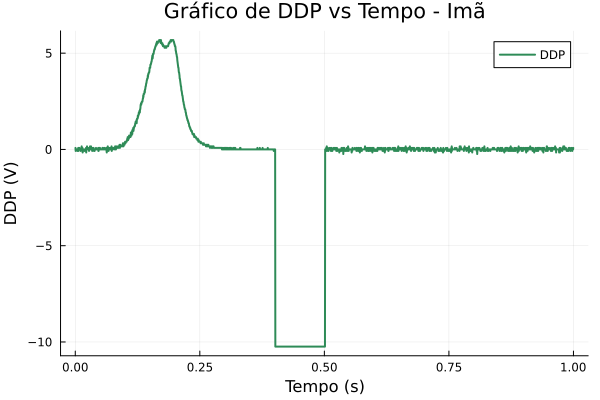
\includegraphics[width=1.0\linewidth]{figuras/grafico_dados1_F0016CH1.png}
\end{figure}

\begin{figure}[H]
    \centering
    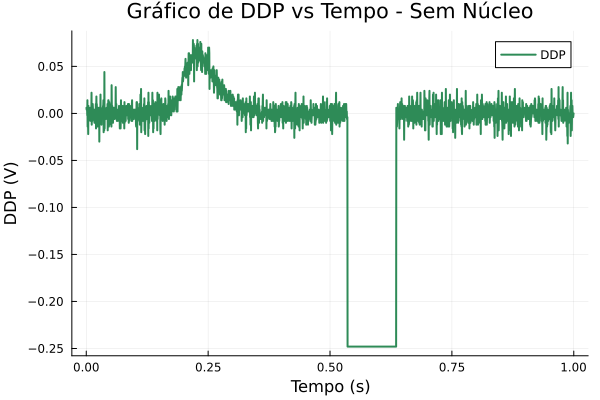
\includegraphics[width=1.0\linewidth]{figuras/grafico_dados2_F0000CH1.png}
\end{figure}

\begin{figure}[H]
    \centering
    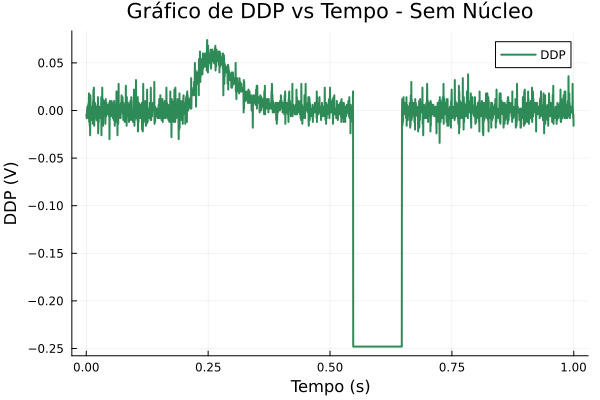
\includegraphics[width=1.0\linewidth]{figuras/grafico_dados2_F0001CH1.png}
\end{figure}

\begin{figure}[H]
    \centering
    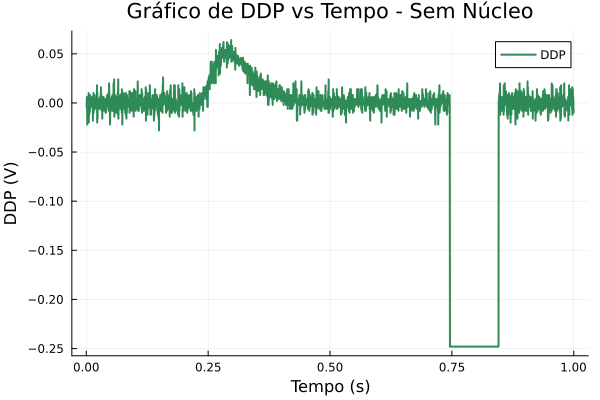
\includegraphics[width=1.0\linewidth]{figuras/grafico_dados2_F0002CH1.png}
\end{figure}

\begin{figure}[H]
    \centering
    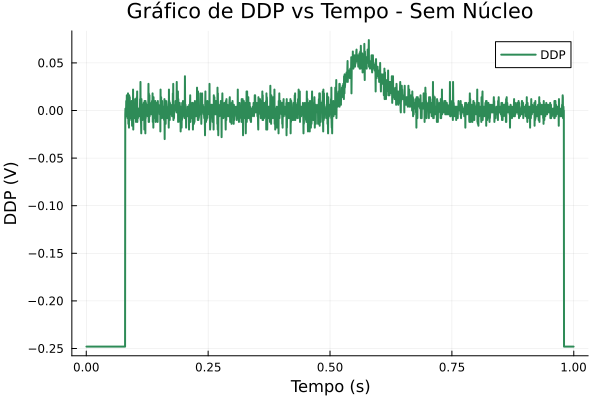
\includegraphics[width=1.0\linewidth]{figuras/grafico_dados2_F0003CH1.png}
\end{figure}

\begin{figure}[H]
    \centering
    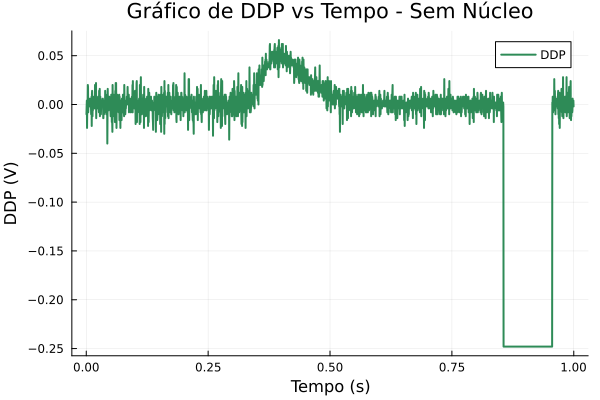
\includegraphics[width=1.0\linewidth]{figuras/grafico_dados2_F0004CH1.png}
\end{figure}

\begin{figure}[H]
    \centering
    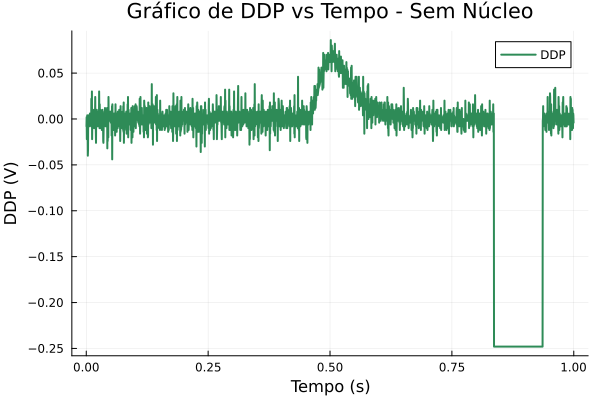
\includegraphics[width=1.0\linewidth]{figuras/grafico_dados2_F0005CH1.png}
\end{figure}

\begin{figure}[H]
    \centering
    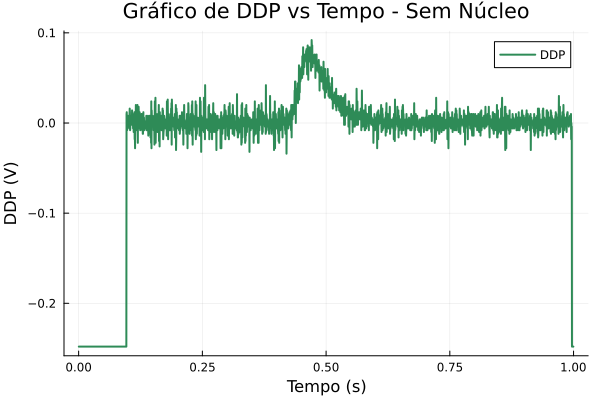
\includegraphics[width=1.0\linewidth]{figuras/grafico_dados2_F0006CH1.png}
\end{figure}

\begin{figure}[H]
    \centering
    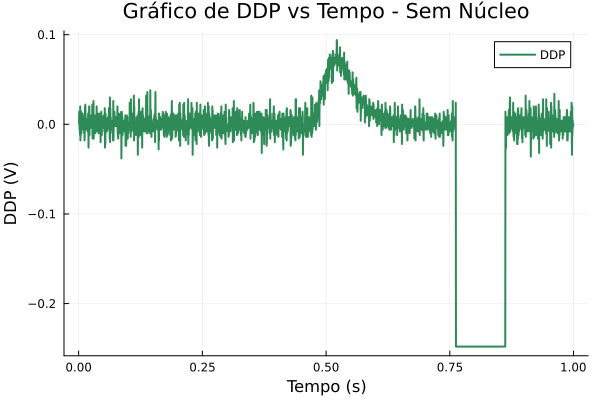
\includegraphics[width=1.0\linewidth]{figuras/grafico_dados2_F0007CH1.png}
\end{figure}

\begin{figure}[H]
    \centering
    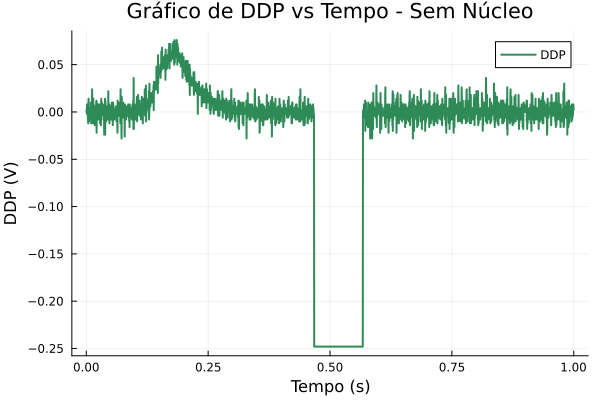
\includegraphics[width=1.0\linewidth]{figuras/grafico_dados2_F0008CH1.png}
\end{figure}

\begin{figure}[H]
    \centering
    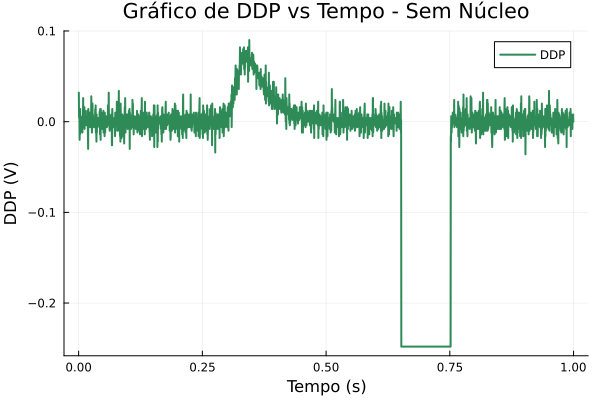
\includegraphics[width=1.0\linewidth]{figuras/grafico_dados2_F0009CH1.png}
\end{figure}

\begin{figure}[H]
    \centering
    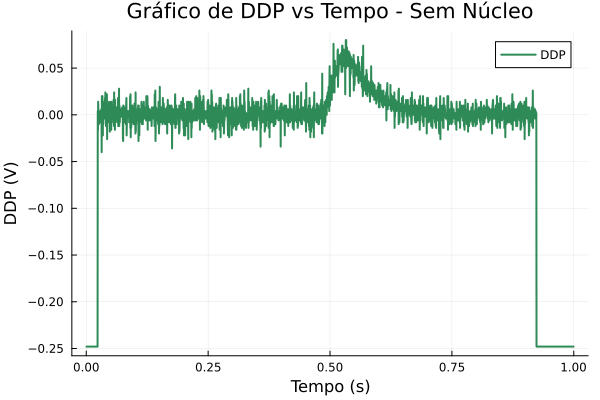
\includegraphics[width=1.0\linewidth]{figuras/grafico_dados2_F0010CH1.png}
\end{figure}

\begin{figure}[H]
    \centering
    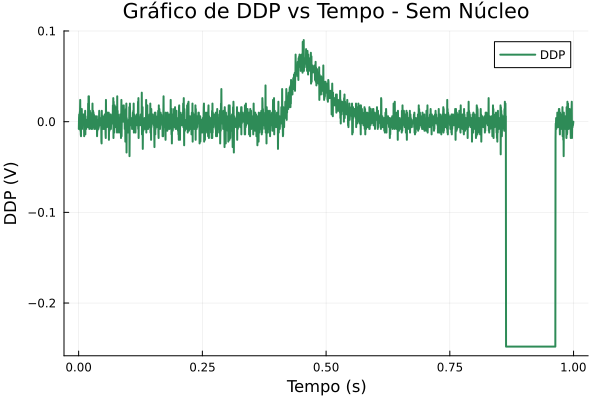
\includegraphics[width=1.0\linewidth]{figuras/grafico_dados2_F0011CH1.png}
\end{figure}

\begin{figure}[H]
    \centering
    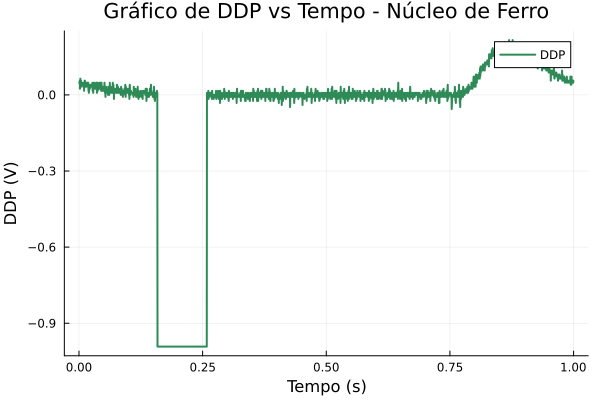
\includegraphics[width=1.0\linewidth]{figuras/grafico_dados3_F0000CH1.png}
\end{figure}

\begin{figure}[H]
    \centering
    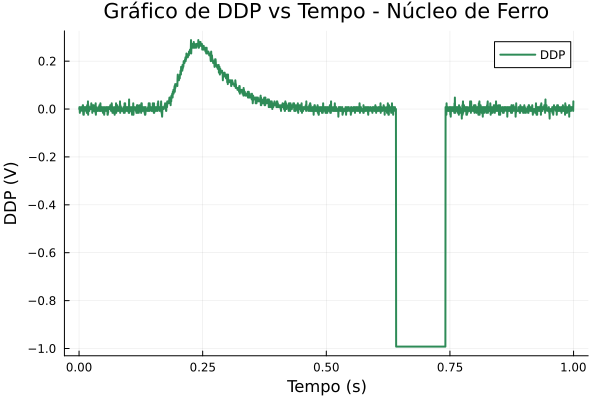
\includegraphics[width=1.0\linewidth]{figuras/grafico_dados3_F0001CH1.png}
\end{figure}

\begin{figure}[H]
    \centering
    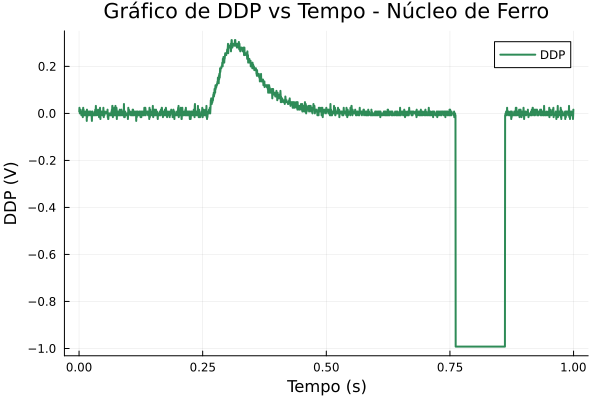
\includegraphics[width=1.0\linewidth]{figuras/grafico_dados3_F0002CH1.png}
\end{figure}

\begin{figure}[H]
    \centering
    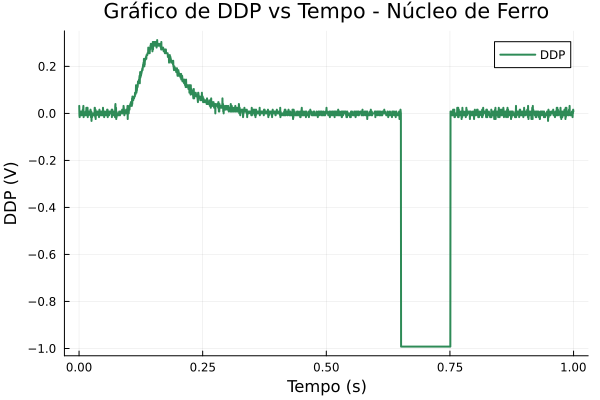
\includegraphics[width=1.0\linewidth]{figuras/grafico_dados3_F0003CH1.png}
\end{figure}

\begin{figure}[H]
    \centering
    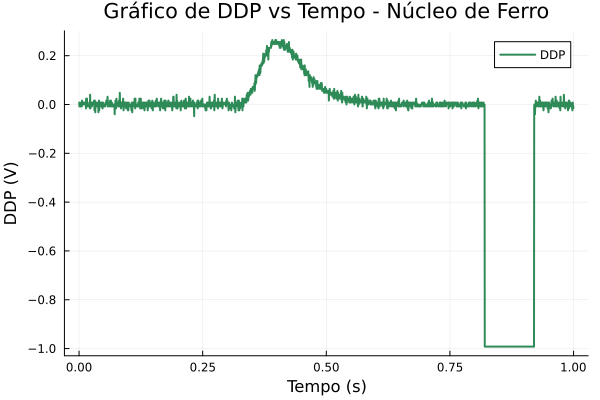
\includegraphics[width=1.0\linewidth]{figuras/grafico_dados3_F0004CH1.png}
\end{figure}

\begin{figure}[H]
    \centering
    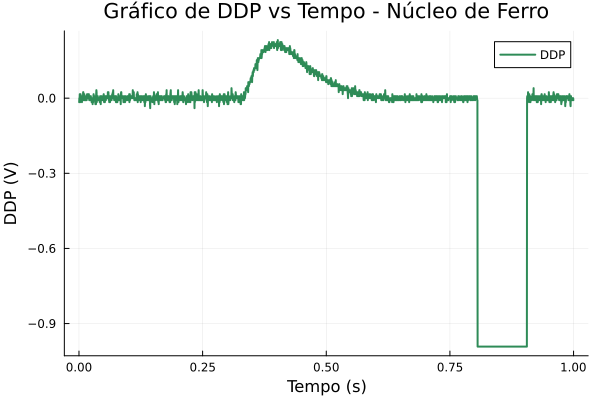
\includegraphics[width=1.0\linewidth]{figuras/grafico_dados3_F0005CH1.png}
\end{figure}

\begin{figure}[H]
    \centering
    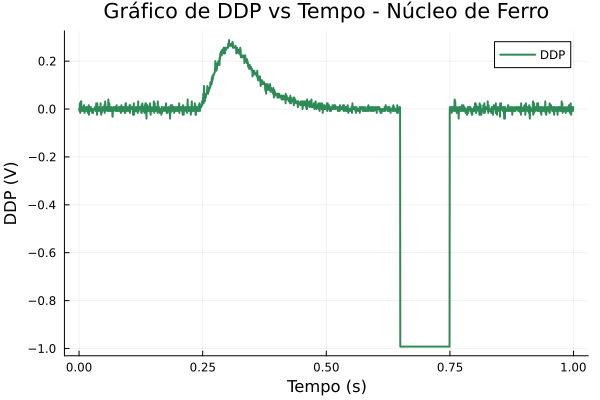
\includegraphics[width=1.0\linewidth]{figuras/grafico_dados3_F0006CH1.png}
\end{figure}

\begin{figure}[H]
    \centering
    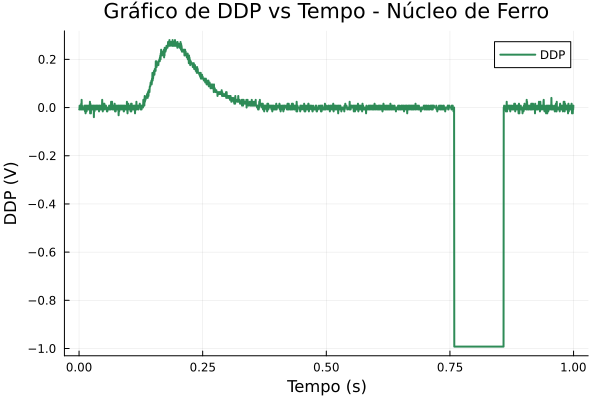
\includegraphics[width=1.0\linewidth]{figuras/grafico_dados3_F0007CH1.png}
\end{figure}

\begin{figure}[H]
    \centering
    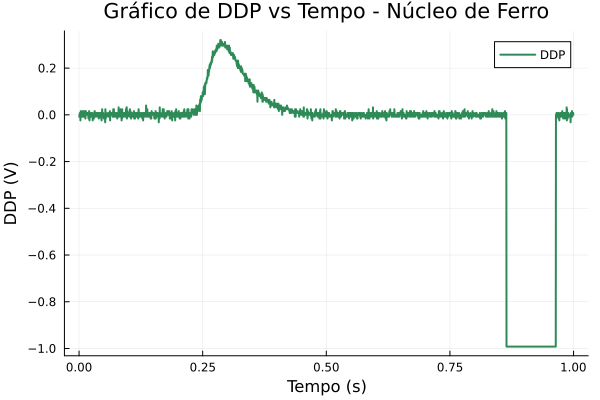
\includegraphics[width=1.0\linewidth]{figuras/grafico_dados3_F0008CH1.png}
\end{figure}

\begin{figure}[H]
    \centering
    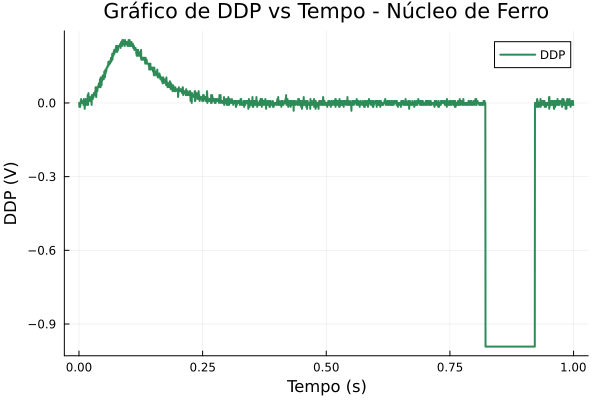
\includegraphics[width=1.0\linewidth]{figuras/grafico_dados3_F0009CH1.png}
\end{figure}

\begin{figure}[H]
    \centering
    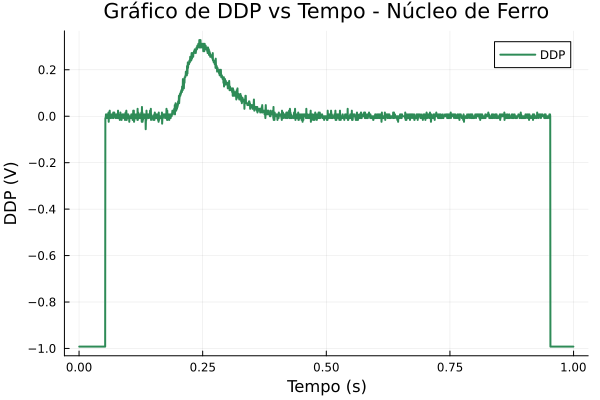
\includegraphics[width=1.0\linewidth]{figuras/grafico_dados3_F0010CH1.png}
\end{figure}

\begin{figure}[H]
    \centering
    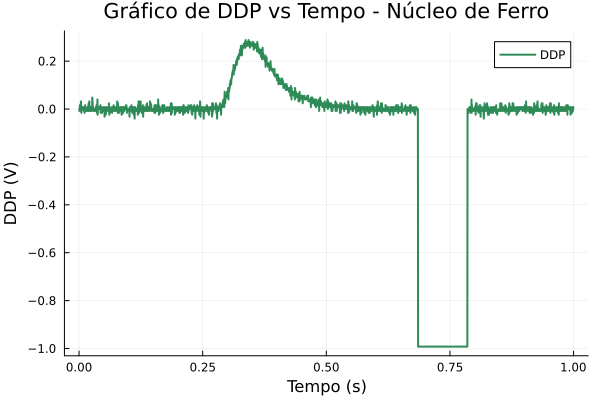
\includegraphics[width=1.0\linewidth]{figuras/grafico_dados3_F0011CH1.png}
\end{figure}

\begin{figure}[H]
    \centering
    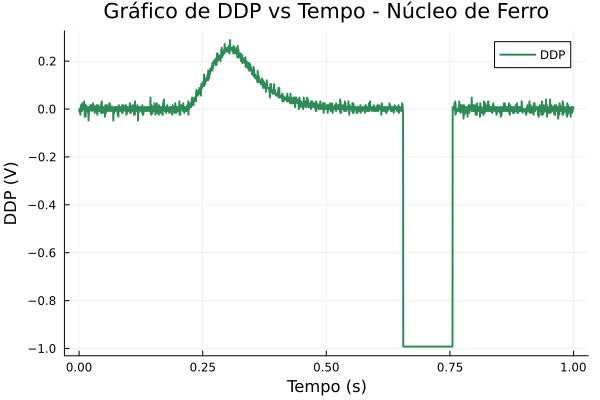
\includegraphics[width=1.0\linewidth]{figuras/grafico_dados3_F0012CH1.png}
\end{figure}

\end{multicols}
\end{center}



\end{document}